\chapter[METHODOLOGY]{Methodology}

\section{General}
The study follows four linked phases. Phase I reviews a representative Draft Final NBC 205:2012 building using the available concrete design-check results. Phase II evaluates the NBC 205:2024 Regular building as the reference model. Phase III extends the comparison to six plan-irregular NBC 205:2024 configurations and considers a separate four-storey height-extension model. Phase IV synthesizes the response measures to interpret the practical applicability limits of NBC 205 RUD provisions.

The structural analyses were carried out in ETABS. The response measures used in the thesis are storey shear, inter-storey drift, CM--CR separation, pushover capacity, performance points, final-step hinge observations, and concrete design-check observations. These quantities are interpreted together because no single parameter provides a complete description of seismic performance.

\section{Analytical Software and Theoretical Basis}
AutoCAD was used to prepare the base architectural/plan layouts for the model configurations. The plan geometry was then represented in ETABS for structural finite-element modelling, assignment of frame and slab elements, and seismic response evaluation. ETABS was used for the structural modelling and seismic-response assessment. The analytical model represents the reinforced-concrete frame members and floor slabs with their defined geometry, material properties, section assignments, gravity loads and seismic loading cases. The investigation combines equivalent-static lateral-force concepts, modal response-spectrum evaluation and nonlinear static pushover analysis. The three approaches serve different purposes and are not treated as interchangeable measures of structural performance.

In the equivalent-static approach, the seismic action is idealized as an equivalent set of horizontal forces acting over the building height. The modal response-spectrum approach relates the building's natural periods and participating modes to the adopted seismic demand spectrum; storey response is then assessed from the modal-analysis results. Nonlinear static pushover analysis applies increasing lateral demand to examine a capacity curve and the progression of the recorded nonlinear response. The performance point, the first global capacity peak and the final recorded hinge state are retained as distinct outputs rather than assumed to occur at the same analysis step \cite{nbc105_2025,atc1996atc40,fema2005fema440}.

\subsection{Model Inputs and Output Interpretation}
The ETABS model inputs comprise plan geometry and storey heights, beam, column and slab sections, concrete and reinforcement properties, gravity and wall loads, the seismic zone factor $Z$, soil classification and NBC 105:2025 demand cases. The material, section and loading assumptions are summarized in the following tables. In the Regular model, the seismic mass includes the full dead, floor-finish and wall-load contributions and 30\% of the floor-live and staircase loads. The response assessment is based on these specified models and loading cases.

The seismic response is evaluated through storey shear, inter-storey drift, centre-of-mass to centre-of-rigidity (CM--CR) separation, modal periods, pushover capacity and performance points. The 2012 reference is assessed through its concrete design checks; the nonlinear comparison concerns the NBC 205:2024 models.



\subsection{Loading and Mass-Source Definition}
The gravity loads adopted in the model setup are summarised in Table~\ref{tab:seq035_load_inputs}. The mass-source expression uses the full dead load and 30\% of the live load. The staircase line loads are presented separately because their application differs from floor-area loads.
\begin{table}[!htbp]\centering
\caption{Gravity-load definitions and nonlinear hinge assignments used in the structural modelling.}\label{tab:seq035_load_inputs}
\normalsize
\begin{tabular}{@{}p{0.49\textwidth}p{0.36\textwidth}@{}}\toprule
Input or assignment & Adopted definition \\\midrule
Floor live load & 2.0 kN/m$^2$ \\
Roof live load & 1.5 kN/m$^2$ \\
Floor finish & 1.25 kN/m$^2$ \\
Peripheral walls & 11.67 kN/m \\
Internal walls & 5.83 kN/m \\
Parapet & 2.20 kN/m \\
Staircase dead line load & 10.48 kN/m \\
Staircase live line load & 6.30 kN/m \\
Seismic mass source & $1.0D+0.30L$ \\
Beam nonlinear hinges & Uncoupled $M_3$ at $0.05L$ and $0.95L$ \\
Column nonlinear hinges & Axial--biaxial interaction ($P$--$M_2$--$M_3$) at $0.05L$ and $0.95L$ \\
\bottomrule\end{tabular}
\end{table}
\subsection{Member Sections and Diaphragm Assumptions}
The 2012 reference and 2024 model groups use the section definitions in Table~\ref{tab:seq035_geometry}. The comparison table describes the adopted model inputs and does not imply that all building geometries are interchangeable.
\begin{table}[!htbp]\centering
\caption{Material, section, slab and diaphragm assignments for the analysed model groups.}\label{tab:seq035_geometry}
\small\begin{tabular}{@{}p{0.22\textwidth}p{0.31\textwidth}p{0.34\textwidth}@{}}\toprule
Parameter & NBC 205:2012 reference & NBC 205:2024 models \\\midrule
Beams & 230 $\times$ 355 mm (Fe415) & 250 $\times$ 355 mm / 250 $\times$ 380 mm (Fe500) \\
Columns & 300 $\times$ 300 mm (Fe500) & 350 $\times$ 350 mm (Fe500) \\
Concrete & M20 & M20 \\
Floor slabs & 125 mm & 125 mm \\
Diaphragm & Rigid & Rigid \\
\bottomrule\end{tabular}
\end{table}

\subsection{Sequence of Modelling and Evaluation}
The work proceeded from the selected plan configurations to the structural-model inputs and then to the response evaluation. First, the plan dimensions and re-entrant layouts were represented in the drawings. Second, beams, columns, slabs, materials and cross-sections were assigned to the ETABS structural models. Third, the documented load patterns, mass-source definition and adopted NBC 105:2025 soil/zone cases were applied. Fourth, the equivalent-static and modal response-spectrum results were examined for force, drift and modal behaviour. Fifth, the available nonlinear static pushover results were compared in terms of capacity, performance point and final recorded hinge evidence. The recorded NBC 205:2012 concrete design checks were evaluated separately from the seven-model 2024 comparison. These phases organize the modelling inputs, analytical outputs and comparative interpretation used throughout the study.

% S03 methods visual, 2026-10-29. Original vector concept—not ETABS case data.
% Panels intentionally omit force/period/capacity numerical ordinates.
\begin{figure}[!htbp]
\centering
\begin{tikzpicture}[x=1cm,y=1cm,>=Latex,font=\scriptsize, every node/.style={inner sep=1.5pt}]
  % three clean panels; use neutral thin strokes for journal/research print
  \foreach \x in {0,5.0,10.0} {\draw[gray!55,rounded corners=3pt] (\x,0) rectangle ++(4.7,4.5);}
  \node[font=\footnotesize\bfseries,align=center] at (2.35,4.10) {(a) Equivalent static};
  \node[font=\footnotesize\bfseries,align=center] at (7.35,4.10) {(b) Response spectrum};
  \node[font=\footnotesize\bfseries,align=center] at (12.35,4.10) {(c) Nonlinear pushover};
  % A: three-level idealized frame, conventional equivalent lateral forces grow upwards
  \draw[thick] (0.82,0.78)--(0.82,3.52) (1.77,0.78)--(1.77,3.52);
  \foreach \y in {1.25,2.20,3.15} {\draw[thick] (.7,\y)--(1.9,\y);}
  \draw[very thick] (.48,.75)--(2.08,.75);
  \draw[->,thick] (1.85,1.25)--(2.58,1.25);
  \draw[->,thick] (1.85,2.20)--(2.91,2.20);
  \draw[->,thick] (1.85,3.15)--(3.30,3.15);
  \node[anchor=west] at (3.05,2.20) {$F_i$};
  \node[align=center] at (2.35,.34) {Static distribution\\of lateral forces};
  % B: mode-shape overlay and idealized response spectrum curve, no numeric reading
  \draw[thick] (5.48,.92)--(5.48,3.31);
  \draw[gray,dashed] (5.48,1.38)--(5.48,2.75);
  \draw[thick] (5.48,.92)..controls (5.73,1.7) and (6.15,2.50)..(6.2,3.31);
  \foreach \y in {1.38,2.24,3.31} {\draw[thin] (5.32,\y)--(6.20,\y);}
  \draw[->] (6.65,1.05)--(9.22,1.05) node[below left] {$T$};
  \draw[->] (6.65,1.05)--(6.65,3.30) node[above] {$S_a$};
  \draw[thick] (6.73,1.15)..controls (7.02,2.90) and (7.20,3.05)..(7.67,2.85)
    --(8.04,2.85)..controls (8.50,2.40) and (8.75,1.65)..(9.13,1.30);
  \node at (7.9,.40) {Modal demands combined};
  % C: nonlinear lateral-force versus roof-displacement conceptual trace
  \draw[->] (10.60,.97)--(14.30,.97) node[below left] {$\Delta$};
  \draw[->] (10.60,.97)--(10.60,3.35) node[above] {$V$};
  \draw[very thick] (10.67,1.05)--(11.80,2.29)..controls (12.45,2.95) and (12.75,3.05)..(13.05,2.94)
    ..controls (13.52,2.72) and (13.84,2.43)..(14.16,2.24);
  \fill (12.38,2.72) circle (1.5pt);
  \node[align=center,anchor=west] at (12.48,3.28) {Illustrative\\capacity};
  \node at (12.35,.40) {Incremental lateral loading};
\end{tikzpicture}
\caption{Conceptual distinction among the equivalent-static, response-spectrum and nonlinear static pushover approaches. The arrows, modal deformation and capacity curve are schematic teaching illustrations, not recorded ETABS response values or code-specific numerical spectra.}
\label{fig:s03_analysis_methods}
\end{figure}

The schematic presented in Figure~\ref{fig:s03_analysis_methods} compares the equivalent-static force distribution, modal response-spectrum concept and nonlinear pushover capacity response.

\section{Research Framework}
\begin{figure}[htbp]
\centering
\begin{tikzpicture}[node distance=0.65cm, every node/.style={font=\small}, phase/.style={draw, rounded corners, align=center, text width=0.78\textwidth, minimum height=0.9cm}, arrow/.style={-Latex, thick}]
\node[phase] (p1) {\textbf{Phase I: Review of representative NBC 205:2012 building}\\Evaluation of concrete design-check results.};
\node[phase, below=of p1] (p2) {\textbf{Phase II: NBC 205:2024 Regular benchmark}\\Evaluation under the adopted NBC 105:2025 demand cases.};
\node[phase, below=of p2] (p3) {\textbf{Phase III: Selected irregular configurations}\\Six plan-irregular three-storey-plus-stair-cover buildings and one separate four-storey-plus-stair-cover height-extension model.};
\node[phase, below=of p3] (p4) {\textbf{Phase IV: Interpretation of RUD applicability}\\Comparison of force, drift, CM--CR separation, capacity, performance-point, hinge, and design-check results.};
\draw[arrow] (p1) -- (p2); \draw[arrow] (p2) -- (p3); \draw[arrow] (p3) -- (p4);
\end{tikzpicture}
\caption{Research framework.}
\label{fig:research_workflow}
\end{figure}

The research framework presented in Figure~\ref{fig:research_workflow} organizes the study from the historical NBC 205:2012 reference through the NBC 205:2024 regular benchmark and irregular-model comparison to the final applicability assessment. This sequence keeps the historical review, regular reference and irregular extensions analytically distinct before their results are synthesized.


\section{Development of Structural Models}
The Regular models used in the principal comparison have three full storeys of 3.0~m each plus a stair-cover level. The plan grid is 12~m by 6~m, comprising three 4~m bays in the X direction and two 3~m bays in the Y direction. Common loading, mass, support, diaphragm, seismic-demand, and analysis procedures were retained for the comparative models; the intended differences are the plan configuration and the detailing associated with the adopted NBC 205 provisions.

The primary comparison contains seven three-storey-plus-stair-cover configurations:
\begin{itemize}[leftmargin=0.8cm,itemsep=0.15em,topsep=0.2em,parsep=0pt]
    \item Regular building
    \item L-type building
    \item L1-type building
    \item L2-type building
    \item T-type building
    \item U-type building
    \item Non-Parallel building
\end{itemize}
Only the separate height-extension model contains four full storeys plus a stair cover. It is not included in the seven-model performance-point tables. This distinction is maintained throughout the thesis so that changes associated with plan configuration are not confused with changes associated with building height.

\subsection{Building Selection and Modelling Considerations}
The reference geometry was selected so that the plan configurations could be compared using a consistent modelling framework. The principal seven models have three complete storeys and a stair-cover level; their differences concern plan arrangement and the resulting geometric irregularity. The separate four-storey-plus-stair-cover case is a height extension and is not pooled with the seven-model performance-point series. The Regular plan is the NBC 205:2024 benchmark, whereas the re-entrant and non-parallel alternatives are comparative test configurations, not buildings automatically eligible for prescriptive RUD design.

The plan drawings and three-dimensional model views document the placement and orientation of the investigated frames. The two-dimensional plan shapes document the plan dimensions and the locations of re-entrant corners; an area-deficit descriptor is defined after the plans, while the non-parallel framing angle is evaluated separately. Geometric area deficit, stiffness eccentricity and code-defined torsional irregularity are not synonymous. The latter requires corresponding end-of-storey displacements and cannot be inferred solely from plan shape or CM--CR separation \cite{nbc205_2024,nbc105_2025}.



\begin{table}[!htbp]
\centering
\caption{Details of the seven investigated plan configurations.}
\label{tab:investigated_models}
\small
\resizebox{\textwidth}{!}{%
\begin{tabular}{@{}llccc p{4.0cm}@{}}
\toprule
Model & Plan type & Storeys & Plan area (m$^2$) & GII (\%) & Special feature \\
\midrule
Regular & Rectangular & 3 + stair cover & 72 & 0.00 & Reference rectangular plan \\
L & L-shaped & 3 + stair cover & 60 & 16.67 & Single re-entrant corner \\
L1 & L-shaped & 3 + stair cover & 48 & 33.33 & Deeper single re-entrant corner \\
L2 & Stepped L-type & 3 + stair cover & 72 & 33.33 & Two-step re-entrant topology \\
T & T-shaped & 3 + stair cover & 48 & 33.33 & Two re-entrant corners \\
U & U-shaped & 3 + stair cover & 60 & 16.67 & Central notch and two re-entrant corners \\
Non-Parallel & Skewed & 3 + stair cover & 84 & 22.22 & Non-parallel framing; $\theta=36.87^{\circ}$ \\
\bottomrule
\end{tabular}
}
\end{table}

% The source floor-plan PDFs are full-page Letter drawings.  CP112 previously used a
% large hard-coded bottom trim, which clipped the lower half of the plans.  These calls
% use tightly cropped vector derivatives so the complete drawings remain visible.
\begin{figure}[H]
\centering
\begin{subfigure}[t]{0.49\textwidth}\centering
\includegraphics[width=\linewidth,keepaspectratio]{figures/ch3/floor_plans/regular_floor_plan.pdf}
\subcaption{Regular}
\end{subfigure}\hfill
\begin{subfigure}[t]{0.49\textwidth}\centering
\includegraphics[width=\linewidth,keepaspectratio]{figures/ch3/floor_plans/l_floor_plan.pdf}
\subcaption{L-shaped}
\end{subfigure}
\caption{Regular and L-shaped floor plans.}
\label{fig:floorplans_regular_l}
\end{figure}

Figure~\ref{fig:floorplans_regular_l} compares the regular reference plan with the first re-entrant L-shaped configuration. The pair provides a direct geometric basis for examining how the introduction of a re-entrant corner changes the plan while the broader modelling framework remains common.


\begin{figure}[H]
\centering
\begin{subfigure}[t]{0.49\textwidth}\centering
\includegraphics[width=\linewidth,keepaspectratio]{figures/ch3/floor_plans/l1_floor_plan.pdf}
\subcaption{L1-shaped}
\end{subfigure}\hfill
\begin{subfigure}[t]{0.49\textwidth}\centering
\includegraphics[width=\linewidth,keepaspectratio]{figures/ch3/floor_plans/l2_floor_plan.pdf}
\subcaption{L2-shaped}
\end{subfigure}
\caption{L1- and L2-shaped floor plans.}
\label{fig:floorplans_l1_l2}
\end{figure}

Figure~\ref{fig:floorplans_l1_l2} shows that the L1 and L2 configurations represent different re-entrant geometries rather than simple scaled copies. Their separate treatment is necessary because equal or similar area-deficit measures do not preserve the location and topology of the missing plan area.


\begin{figure}[H]
\centering
\begin{subfigure}[t]{0.49\textwidth}\centering
\includegraphics[width=\linewidth,keepaspectratio]{figures/ch3/floor_plans/t_floor_plan.pdf}
\subcaption{T-shaped}
\end{subfigure}\hfill
\begin{subfigure}[t]{0.49\textwidth}\centering
\includegraphics[width=\linewidth,keepaspectratio]{figures/ch3/floor_plans/u_floor_plan.pdf}
\subcaption{U-shaped}
\end{subfigure}
\caption{T- and U-shaped floor plans.}
\label{fig:floorplans_t_u}
\end{figure}

Figure~\ref{fig:floorplans_t_u} presents two configurations with multiple re-entrant corners. The T- and U-shaped plans distribute the removed area differently, which can alter stiffness distribution, eccentricity and deformation demand even when a single area-based index is similar.


\begin{figure}[H]
\centering
\includegraphics[width=0.86\textwidth,height=0.42\textheight,keepaspectratio]{figures/ch3/floor_plans/non_parallel_floor_plan.pdf}
\caption{Non-Parallel floor plan.}
\label{fig:floorplan_nonparallel}
\end{figure}

Figure~\ref{fig:floorplan_nonparallel} shows the skewed framing arrangement of the Non-Parallel configuration. Its geometric mechanism differs from the re-entrant-corner cases, so the non-parallel angle is retained separately from the area-deficit GII.

\FloatBarrier

\subsection{Geometric Irregularity Index Definition}
For the plan comparison, GII is the percentage plan-area deficit relative to the corresponding bounding rectangle. Figure~\ref{fig:gii_definition} shows the definition schematically for a re-entrant plan. The missing/re-entrant area is a geometric descriptor only; the location and topology of the missing area are retained separately through the plan type, re-entrant projections and corner count.

\begin{figure}[!htbp]
\centering
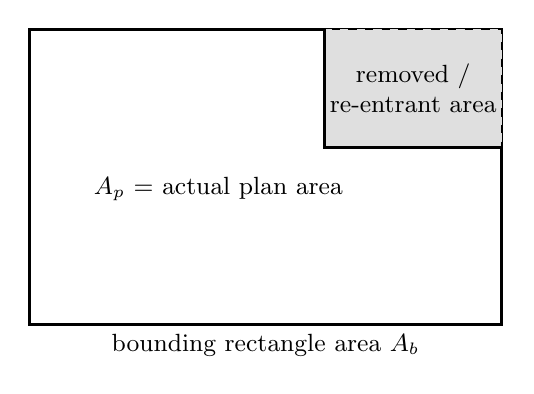
\begin{tikzpicture}[scale=0.75,font=\small]
\draw[very thick] (0,0) rectangle (8,5);
\fill[gray!25] (5,3) rectangle (8,5);
\draw[very thick] (0,0)--(8,0)--(8,3)--(5,3)--(5,5)--(0,5)--cycle;
\draw[dashed] (0,0) rectangle (8,5);
\node at (3.2,2.3) {$A_p$ = actual plan area};
\node[align=center] at (6.5,4.0) {removed /\\re-entrant area};
\node[below] at (4,0) {bounding rectangle area $A_b$};
\end{tikzpicture}
\caption{Geometric Irregularity Index definition.}
\label{fig:gii_definition}
\end{figure}

Figure~\ref{fig:gii_definition} defines GII as the percentage difference between the bounding-rectangle area and the actual plan area. The index therefore measures plan-area deficit only; it does not identify the location, direction or topology of the irregular portion.


\begin{table}[!htbp]
\centering
\caption{Geometric descriptors used with GII.}
\label{tab:gii_geometry}
\scriptsize
\resizebox{\textwidth}{!}{%
\begin{tabular}{@{}lcccccccc@{}}
\toprule
Model & $A_p$ & $A_b$ & GII & corners & max $R_x$ & max $R_y$ & aspect & $\theta$ \\
 & (m$^2$) & (m$^2$) & (\%) & & (\%) & (\%) & ratio & (deg) \\
\midrule
Regular & 72 & 72 & 0.00 & 0 & 0.00 & 0.00 & 2.00 & -- \\
L & 60 & 72 & 16.67 & 1 & 33.33 & 50.00 & 2.00 & -- \\
L1 & 48 & 72 & 33.33 & 1 & 66.67 & 50.00 & 2.00 & -- \\
L2 & 72 & 108 & 33.33 & 2 & 33.33 & 33.33 & 1.33 & -- \\
T & 48 & 72 & 33.33 & 2 & 33.33 & 50.00 & 2.00 & -- \\
U & 60 & 72 & 16.67 & 2 & 33.33 & 50.00 & 2.00 & -- \\
Non-Parallel & 84 & 108 & 22.22 & 0 & 0.00 & 0.00 & 1.33 & 36.87 \\
\bottomrule
\end{tabular}
}
\par\smallskip
\begin{minipage}{0.97\textwidth}\footnotesize
$R_x$ and $R_y$ are geometric re-entrant projection descriptors used in the geometric calculations; they are kept distinct from GII. The Non-Parallel angle is an additional study descriptor and is not folded into GII.
\end{minipage}
\end{table}
\FloatBarrier


% SEQ032: paired, uniformly sized model images with original source files.
\newcommand{\saugatMethodPanel}[4]{%
\begin{minipage}[t]{0.485\textwidth}\centering
\begin{minipage}[c][0.19\textheight][c]{\linewidth}\centering
\includegraphics[width=\linewidth,height=0.18\textheight,keepaspectratio]{#1}
\end{minipage}
\caption{#2 building model.}\label{#3}
{\small\raggedright #4\par}
\end{minipage}}

\begin{figure}[p]\centering
\saugatMethodPanel{figures/ch4/final_final_original/models/SRC-FF-IMG-001_Regular_Building.png}{Regular}{fig:method_regular_model}{The regular model provides the reference configuration for the plan-comparison series.}
\hfill
\saugatMethodPanel{figures/ch4/final_final_original/models/SRC-FF-IMG-002_L_Building.png}{L-type}{fig:method_l_model}{The L-shaped arrangement introduces one re-entrant corner.}

\medskip
\saugatMethodPanel{figures/ch4/final_final_original/models/SRC-FF-IMG-003_L1_Building.png}{L1-type}{fig:method_lone_model}{L1 represents a deeper re-entrant configuration than the first L-shaped case.}
\hfill
\saugatMethodPanel{figures/ch4/final_final_original/models/SRC-FF-IMG-004_L2_Building.png}{L2-type}{fig:method_ltwo_model}{The stepped L2 plan retains its separate re-entrant topology.}
\end{figure}

\begin{figure}[p]\centering
\saugatMethodPanel{figures/ch4/final_final_original/models/SRC-FF-IMG-005_T_Building.png}{T-type}{fig:method_t_model}{The T-shaped layout contains re-entrant corners on opposing sides of the plan.}
\hfill
\saugatMethodPanel{figures/ch4/final_final_original/models/SRC-FF-IMG-006_U_Building.png}{U-type}{fig:method_u_model}{The U-shaped configuration includes a central notch and two re-entrant corners.}

\medskip
\saugatMethodPanel{figures/ch4/final_final_original/models/SRC-FF-IMG-007_Non_Parallel_Building.png}{Non-Parallel}{fig:method_np_model}{The non-parallel framing arrangement is evaluated separately from the re-entrant plans.}
\hfill
\saugatMethodPanel{figures/ch4/final_final_original/models/SRC-FF-IMG-008_4_Storey_Regular_Building.png}{separate four-storey Regular extension}{fig:method_fourstorey_model}{The four-storey height extension is not part of the seven-model performance-point series.}
\end{figure}
\FloatBarrier

\subsection{NBC 205:2012 Detailing Reference}
The NBC~205:2012 dimensional illustration is reproduced in Appendix~\ref{appx:reviewer_nbc205_illustration}, explicitly distinguished from the actual material, member-section and loading assumptions tabulated for the ETABS comparison. The code illustrations and the model input parameters are examined separately to distinguish published detailing provisions from the numerical assumptions used in the structural analysis.

\subsection{Model Geometry and Section Checks}
The following model screenshots document the geometry restrictions and member-section selection used during the setup of the structural comparisons. They supplement, but do not replace, the quantitative section assignments and design-check results.
\begin{figure}[!htbp]
\centering
\includegraphics[width=0.83\textwidth,height=0.27\textheight,keepaspectratio]{figures/ch3/seq035/model_validation/NBC 205_2012 Building Restrictions .jpg}
\caption{Building-configuration restrictions associated with NBC 205:2012.}
\par\vspace{3pt}{\small\raggedright The restrictions summarize the plan and height conditions used to establish the reference building geometry; the model response is evaluated separately.\par}
\end{figure}
\begin{figure}[!htbp]
\centering
\includegraphics[width=0.83\textwidth,height=0.27\textheight,keepaspectratio]{figures/ch3/seq035/model_validation/NBC 205_2024 Building Restrictions .jpg}
\caption{Building-configuration restrictions associated with NBC 205:2024.}
\par\vspace{3pt}{\small\raggedright The plan-configuration limits are shown for comparison with the investigated regular and irregular arrangements and do not constitute an automatic design approval.\par}
\end{figure}
\begin{figure}[!htbp]
\centering
\includegraphics[width=0.83\textwidth,height=0.27\textheight,keepaspectratio]{figures/ch3/seq035/model_validation/NBC205_2012_Beam Section Choose Part 1.jpg}
\caption{Beam section selection for the 2012 reference.}
\par\vspace{3pt}{\small\raggedright The section-selection view documents the beam dimensions considered for the earlier reference frame.\par}
\end{figure}
\begin{figure}[!htbp]
\centering
\includegraphics[width=0.83\textwidth,height=0.27\textheight,keepaspectratio]{figures/ch3/seq035/model_validation/NBC205_2024_Beam Section Choose Part 1.jpg}
\caption{Beam section selection for the 2024 models.}
\par\vspace{3pt}{\small\raggedright The beam section choices are compared with the tabulated member properties used to define the analytical models.\par}
\end{figure}
\begin{figure}[!htbp]
\centering
\includegraphics[width=0.83\textwidth,height=0.27\textheight,keepaspectratio]{figures/ch3/seq035/model_validation/Column Section_NBC205_2012.jpg}
\caption{Column section selection for the 2012 reference.}
\par\vspace{3pt}{\small\raggedright The column section view identifies the reference geometry used in the earlier-code model.\par}
\end{figure}
\begin{figure}[!htbp]
\centering
\includegraphics[width=0.83\textwidth,height=0.27\textheight,keepaspectratio]{figures/ch3/seq035/model_validation/Column Section_NBC205_2024 part 1.jpg}
\caption{Column section selection for the 2024 models.}
\par\vspace{3pt}{\small\raggedright The column section view documents the model geometry considered for the newer configurations; verification of reinforcement demands requires the corresponding design results.\par}
\end{figure}
\FloatBarrier

\subsection{Structural Model Comparison Framework}
The Phase I model follows Draft Final NBC 205:2012 and is evaluated using the available concrete design-check results. The Phase II Regular model follows NBC 205:2024 and provides the reference for the performance-based assessment \cite{nbc205_2012,nbc205_2024}. Five NBC 105:2025 demand cases are considered for the 2024 models: Soil Type C with $Z=0.25$, $0.30$, $0.35$, and $0.40$, and Soil Type D with $Z=0.35$ \cite{nbc105_2025}.

\section{Seismic Parameters}
The adopted soil categories are Soil Type C and Soil Type D. The seismic zone factors considered are $Z=0.25$, $0.30$, $0.35$, and $0.40$. The matched demand cases used in the comparative results are Soil Type C at each of the four zone factors and Soil Type D at $Z=0.35$.


\subsection{Material, Section and Loading Inputs}
The seven ETABS models use M20 concrete, HYSD415/HYSD500 reinforcement, 125~mm floor slabs and the loading patterns presented below. Material properties, section dimensions and gravity and seismic actions are summarized in Tables~\ref{tab:material_properties}--\ref{tab:load_patterns}.

\begin{table}[!htbp]
\centering
\caption{Principal material properties used in the ETABS models.}
\label{tab:material_properties}
\small
\resizebox{\textwidth}{!}{%
\begin{tabular}{@{}lcccc@{}}
\toprule
Material & $f_c$/$f_y$ (MPa) & $E$ (MPa) & $\nu$ & Structural application \\
\midrule
M20 concrete & $f_c=20$ & 22360.68 & 0.20 & RC beams, columns and slabs \\
HYSD415 rebar & $f_y=415$ & 200000 & -- & Longitudinal/confining reinforcement definitions \\
HYSD500 rebar & $f_y=500$ & 200000 & -- & Longitudinal/confining reinforcement definitions \\
\bottomrule
\end{tabular}
}
\end{table}

\begin{table}[!htbp]
\centering
\caption{Principal section families used in the seven ETABS models.}
\label{tab:section_properties}
\small
\resizebox{\textwidth}{!}{%
\begin{tabular}{@{}lll@{}}
\toprule
Element & Section type & Nominal size \\
\midrule
Beam & M20 rectangular beam & 250$\times$355 mm and 250$\times$380 mm \\
Column & M20 rectangular column & 350$\times$350 mm; selected stair columns 400$\times$400 mm \\
Floor slab & M20 shell/slab & 125 mm \\
\bottomrule
\end{tabular}
}
\end{table}

\begin{table}[!htbp]
\centering
\caption{Load patterns and seismic cases used in the seven-model analyses.}
\label{tab:load_patterns}
\small
\begin{tabular}{@{}lp{8.5cm}@{}}
\toprule
Group & Model loading \\
\midrule
Gravity & Dead (self-weight), Floor Live, Roof Live, Staircase, Floor Finish \\
Wall & Peripheral Wall, Internal Wall, Parapet Wall \\
Seismic & EQx ULS, EQy ULS, EQx SLS, EQy SLS; 5\% accidental eccentricity was specified in the Regular model \\
Mass source & Dead + floor finish + wall loads at full factor, with 0.30 of Floor Live and Staircase in the Regular model \\
\bottomrule
\end{tabular}
\end{table}

\subsection{NBC 105:2025 Response Spectrum Basis}
The modal response-spectrum method uses the NBC 105:2025 spectral-shape-factor definition. Figure~\ref{fig:nbc105_mrsm_spectrum} reproduces the official code figure used as the spectral reference; the study demand cases use Soil Types C and D and the zone factors listed above.
\begin{figure}[!htbp]
\centering
\includegraphics[width=0.86\textwidth]{figures/ch1/nbc105_2025_mrsm_spectrum.png}
\caption{NBC 105:2025 response spectrum (Source: NBC 105:2025 \cite{nbc105_2025}).}
\label{fig:nbc105_mrsm_spectrum}
\end{figure}

The response-spectrum plot in Figure~\ref{fig:nbc105_mrsm_spectrum} shows the code spectral-shape basis used for modal response-spectrum analysis. The study applies this code-defined demand framework to the selected soil classes and seismic zone factors rather than deriving a separate project-specific response spectrum \cite{nbc105_2025}.

\FloatBarrier

\subsection{Modal Analysis and Mass-Participation Extraction}
Modal analysis was evaluated for the Regular, L, L1, L2, T, U and Non-Parallel building configurations. Twelve modes were considered for each seismic demand case. The main response measures are natural period, frequency, translational modal participation in the X and Y directions (UX and UY), and cumulative mass participation (SumUX and SumUY). These parameters indicate the relative contributions of the vibration modes to the building response.

The modal comparison in Chapter~4 uses Soil Type C at $Z=0.40$ to maintain a consistent demand case across the seven building configurations. The analyses also consider the remaining soil and seismic-zone combinations described in the Seismic Parameters section.

\begin{table}[!htbp]
\centering
\caption{Modal quantities extracted from the seven ETABS modal-participation workbooks.}
\label{tab:modal_extraction_fields}
\small
\begin{tabular}{@{}p{3.5cm}p{4.0cm}p{6.1cm}@{}}
\toprule
Quantity & Workbook field & Use in this study \\
\midrule
Modal period & Period & $T_1$, $T_2$, and $T_3$ are reported for the matched seven-model comparison. \\
Per-mode translational participation & UX, UY & Identifies the dominant X- and Y-translational modes. \\
Cumulative translational participation & SumUX, SumUY & Checks how many modes are required to exceed 90\% cumulative mass participation in each horizontal direction. \\
Frequency information & Frequency, CircFreq, Eigenvalue & Retained in the normalized electronic dataset for future verification. \\
\bottomrule
\end{tabular}
\end{table}

\FloatBarrier


\section{NBC 105:2025 Response Evaluation}
Storey shear and inter-storey drift are evaluated for the seven principal configurations under the adopted demand cases. The ULS drift ratio is checked against the NBC 105:2025 limit of 0.025. Storey shear is used to compare the distribution of lateral-force demand among the configurations, while drift is used to compare deformation demand \cite{nbc105_2025}.

\section{CM--CR Separation}
The centre-of-mass and centre-of-rigidity coordinates are used to calculate the resultant CM--CR separation at the available floor levels. The principal quantities considered are the centre-of-mass coordinates, centre-of-rigidity coordinates, and resultant separation. CM--CR separation is used as a descriptive indicator of mass--stiffness eccentricity and is interpreted together with the other response measures.

\begin{figure}[!htbp]
\centering
\includegraphics[width=0.82\textwidth,height=0.34\textheight,keepaspectratio]{figures/ch3/seq035/typical_eccentric_cm_cr.jpg}
\caption{Typical single eccentric system showing center of mass (CM) and eccentric center of rigidity (CR).}
\label{fig:typical_eccentric_cm_cr}
\end{figure}
The schematic illustrates how an offset between the centre of mass and the centre of rigidity introduces eccentricity in a structural plan. It is a conceptual representation rather than a plan or measured displacement from any of the seven models.


\section{Nonlinear Static Pushover Analysis}
Nonlinear static pushover analysis is used to compare lateral capacity and demand-state response. Capacity curves are considered up to the first global peak for consistent presentation. Performance-point base shear and roof displacement are interpreted separately from the first-peak pushover capacity. Final-step hinge observations are also reported separately and are not assumed to represent the hinge state at the performance point unless such a state is directly available from the analysis output \cite{atc1996atc40,fema2005fema440,asce2017asce41}.

The outputs considered from the pushover analysis are:
\begin{itemize}[leftmargin=0.8cm,itemsep=0.15em,topsep=0.2em,parsep=0pt]
    \item capacity curves;
    \item performance-point base shear and roof displacement;
    \item first-peak base shear and corresponding displacement; and
    \item final recorded hinge state.
\end{itemize}

\subsection{Pushover Response Measures}
The nonlinear static pushover comparison considers X- and Y-direction capacity curves and performance-point outputs for all seven configurations under the five matched seismic demand cases. The recorded results include performance-point base shear and roof displacement, capacity at the first global peak, and final-step hinge-formation images.

Capacity curves are compared through their first global peak. Performance-point response is interpreted separately from peak capacity, and the final-step hinge patterns are discussed only at their recorded analysis stages rather than being treated as performance-point hinge states.


\section{Comparative Evaluation}
The principal comparison uses storey shear, inter-storey drift, CM--CR separation, pushover capacity, performance-point response, hinge behaviour, and concrete design-check observations. The 2012 building is reviewed from the available design-check results, the 2024 Regular building is used as the reference, and the selected irregular models are compared with that reference. The separate four-storey height-extension model is treated independently of the seven-model plan-configuration comparison. The separate four-storey model is interpreted through its design-check findings and is not used to quantify a height effect on storey-force distribution.

For the geometric comparison, plan irregularity is represented by the Geometric Irregularity Index (GII), calculated as the plan-area deficit relative to the corresponding bounding rectangle:
\begin{equation}
\mathrm{GII}=\left(1-\frac{A_p}{A_b}\right)\times 100,
\label{eq:gii_plan_deficit}
\end{equation}
\ifdefined\PURegisterEquationEntry
\PURegisterEquationEntry{Geometric Irregularity Index}
\fi
where $A_p$ is the actual plan area and $A_b$ is the area of the corresponding bounding rectangle. GII is expressed as a percentage and is compared with selected performance-point response parameters. For the Non-Parallel configuration, the non-parallelism angle $\theta=36.87^{\circ}$ is retained as an additional geometric descriptor. The comparison is descriptive; configurations with the same GII are retained as separate cases and no universal relationship is inferred from the limited model set.
